\section{Contraction-derived adaptation: proofs and extensions}
\label{app:adaptive}\label{app:composite}
The results concern the system and domain explicitly specified in
Appendix~\ref{sec:gen-theory}. Geodesic cancellation establishes adaptive
tracking of the nominal physical response to the same supplied commands.
The certificate concerns the robot and low-level execution controller;
it does not certify the full VLA feedback loop or differential dynamics
of the augmented adaptive system.

\subsection{First variation of the geodesic half-energy}
\label{app:first-variation}
Fix a time $t$ within a command-continuity interval in a certified smooth
mode, and the minimizing geodesic $c(s)$ in
\eqref{eq:contraction-energy}. For a small positive increment $h$, flow
each point under $F_{\rm exec}$ with the same supplied VLA command signal:
$c_h(s)=\phi^r_{t+h,t}(c(s))$. The signal is fixed for every virtual
trajectory. The curve and its short-time images remain in that smooth
domain; hybrid crossings require the separate bounds in
Appendix~\ref{app:history-partition}. The tangent variation obeys
$\partial_h(c_h)_s=A_{\rm exec}(c_h,r(t+h),t+h)(c_h)_s$.
No policy derivative enters this variation. Write its energy as
$\mathcal E(h)=\frac12\int_0^1(c_h)_s^\top M_c(c_h,t+h)(c_h)_s\,ds$.
Differentiating at $h=0$ gives
\begin{align}
 \mathcal E'(0)&=\frac12\int_0^1c_s^\top
 \big(\partial_tM_c+\partial_{F_{\rm exec}}M_c+A_{\rm exec}^\top M_c+M_cA_{\rm exec}\big)c_s\,ds
 \nonumber\\[-1mm]
 &\le-\lambda\int_0^1c_s^\top M_cc_s\,ds
 =-\lambda X^2.
 \label{eq:geodesic-nominal-proof}
\end{align}
The minimizing energy between the transported endpoints is no larger
than that of this transported curve. They agree at $h=0$, so the same
upper derivative bound applies to the squared distance when both
endpoints follow $F_{\rm exec}$ under the same supplied $r(t)$.

For completeness, with the start point fixed, perturb the endpoint by
$\delta\xi$ and let $\delta c(s)$ be the induced curve variation.
The first variation at a minimizing geodesic is
\begin{align}
 \delta V_\xi
 &=\left[c_s^\top M_c\,\delta c\right]_0^1+
 \int_0^1\left[\frac{\partial L}{\partial c}
       -\frac{d}{ds}\frac{\partial L}{\partial c_s}\right]^\top
       \delta c\,ds
 =p_\xi^\top\delta\xi,\qquad
 L=\tfrac12c_s^\top M_c(c,t)c_s.
 \label{eq:geodesic-first-variation}
\end{align}
The interior term vanishes by the geodesic Euler--Lagrange equation;
$\delta c(0)=0$ and $\delta c(1)=\delta\xi$. Therefore the actual endpoint
perturbation $-B_\theta\tilde\theta+d_{\rm eff}$ adds exactly
$-\sigma_{\rm exec}^\top\tilde\theta+p_\xi^\top d_{\rm eff}$ to the nominal
upper derivative. This proves \eqref{eq:gen-storage}. The smooth squared
distance assumption makes this a classical endpoint derivative; writing
$D^+$ also accommodates norm comparisons at zero. We have not assumed
smoothness through a cut locus. For piecewise-continuous commands, the
flow inequality applies almost everywhere and is concatenated across
command changes. If $\xi$, $\xi^{\rm nom}$, and $M_c$ are continuous, these
changes cause no energy jump because the metric is command-independent.

Since the minimizing geodesic has constant metric speed on $[0,1]$,
$c_s(1)^\top M_c(\xi,t)c_s(1)=X^2$. Hence
\begin{equation}
 \|M_c(\xi,t)^{-1/2}p_\xi\|=X,\qquad
 |p_\xi^\top d_{\rm eff}|\le X\|d_{\rm eff}\|_{M_c(\xi,t)},\qquad
 |\sigma_{\rm exec}^\top\tilde\theta|\le L_BXZ.
 \label{eq:geodesic-endpoint-bounds}
\end{equation}
The last inequality uses \eqref{eq:gen-coupling} and
$Z=\|\tilde\theta\|_{\Gamma^{-1}}$. The metric lower bound also gives
$X\ge\sqrt{\underline m}\|\xi-\xi^{\rm nom}\|$, since the Euclidean length of any
connecting curve is at least the endpoint distance.

\subsection{Projection, cancellation, and the composite bound}
\label{app:gen-proof}
Let $\Theta$ be fixed, closed, and convex, with initial estimate and true
parameter in $\Theta$. Define $\operatorname{Proj}^{\Gamma}_\Theta(h,v)$
as the metric projection of $v$ onto the tangent cone $T_\Theta(h)$ in
the $\Gamma^{-1}$ norm. Assume the resulting projected differential
equation admits an absolutely continuous solution between jumps.
The weighted tangent-cone projection yields a normal
$n=\Gamma^{-1}(v-\operatorname{Proj}^{\Gamma}_\Theta(h,v))\in N_\Theta(h)$,
where $n^\top(\theta-h)\le0$ for all $\theta\in\Theta$. Taking
$h=\hat\theta$ and $\theta=\theta^*$ proves
\begin{equation}
 \tilde\theta^\top\Gamma^{-1}
 [\operatorname{Proj}^{\Gamma}_\Theta(\hat\theta,v)-v]\le0.
 \label{eq:gen-projection}
\end{equation}
This parameter projection does not ensure feasible actuator commands;
allocation must enforce the physical input constraints separately.

With $V_\theta=\tilde\theta^\top\Gamma^{-1}\tilde\theta/2$, the update
\eqref{eq:gen-law} and \eqref{eq:gen-projection} imply, almost everywhere,
\begin{equation}
 \dot V_\theta\le\kappa\tilde\theta^\top\sigma_{\rm exec}
 -k_c\tilde\theta^\top H_I\tilde\theta
 +k_c\tilde\theta^\top\epsilon_I
 -\tilde\theta^\top\Gamma^{-1}\dot\theta^*.
 \label{eq:gen-parameter-proof}
\end{equation}
Thus $V=V_\xi+V_\theta$ obeys the derived cancellation identity
\begin{align}
 D^+V\le{}&-\lambda X^2-(1-\kappa)\sigma_{\rm exec}^\top\tilde\theta
 -k_c\tilde\theta^\top H_I\tilde\theta+p_\xi^\top d_{\rm eff}\nonumber\\
 &+k_c\tilde\theta^\top\epsilon_I
 -\tilde\theta^\top\Gamma^{-1}\dot\theta^*.
 \label{eq:gen-joint-dissipation}
\end{align}
At $\kappa=1$ the cross term cancels, which determines the positive sign
and endpoint form of the tracking term in the law. With
$\sqrt{\gamma_-}Z\le\|\tilde\theta\|\le\sqrt{\gamma_+}Z$,
$\|\Gamma^{-1/2}\dot\theta^*\|\le\nu/\sqrt{\gamma_-}$,
and the bounds in Theorem~\ref{thm:gen-adaptive},
\begin{equation}
 D^+V\le-\beta(X^2+Z^2)+\bar d_MX+
 \left(k_c\sqrt{\gamma_+}\bar\epsilon_I+\nu/\sqrt{\gamma_-}\right)Z
 \le-2\beta V+Q\sqrt{2V}.
 \label{eq:gen-V-bound}
\end{equation}
For $W=\sqrt{2V}>0$, divide by $W$. At zero, regularize the norm by
$\sqrt{2V+\eta}$ and let $\eta\downarrow0$ to obtain the same upper
comparison. Integrating $D^+W\le-\beta W+Q$ proves
\eqref{eq:gen-envelope}. Euclidean component bounds follow from metric
bounds, and tube containment is the standard first-exit argument under
all stated domain conditions. This proves Theorem~\ref{thm:gen-adaptive}.
If $\hat\sigma_{\rm exec}=\sigma_{\rm exec}+\epsilon_\sigma$ is used, add
$\kappa\tilde\theta^\top\epsilon_\sigma$ to
\eqref{eq:gen-joint-dissipation}; its norm bound gives exactly the extra
forcing specified in Appendix~\ref{sec:gen-theory}. A metric inequality
with certified defect $+2\delta M_c$ similarly replaces $\lambda$ by
$\lambda-\delta$ when this rate remains positive.

\paragraph{Projected observer contraction requires a common data stream.}
For two prediction-only solutions $h_1,h_2$, write
$\dot h_i=k_c\Gamma(b_I-H_Ih_i)-\Gamma n_i$ with
$n_i\in N_\Theta(h_i)$. Normal-cone monotonicity gives
$(h_1-h_2)^\top(n_1-n_2)\ge0$. Therefore
\begin{equation}
 \frac{d}{dt}\frac12\|h_1-h_2\|_{\Gamma^{-1}}^2
 \le-k_c(h_1-h_2)^\top H_I(h_1-h_2)
 \le-k_c\mu\gamma_-\|h_1-h_2\|_{\Gamma^{-1}}^2.
 \label{eq:projected-observer-contraction}
\end{equation}
This proof applies to the projected differential equation without
classical Jacobians at active faces. It compares observers driven by
identical exogenous $H_I,b_I$; it does not discard their state dependence
in the actual robot loop.

\subsection{Prediction-only comparison and the weighted extension}
\label{app:prediction-proof}
For $\kappa=0$, divide \eqref{eq:gen-storage} by $X>0$ and
\eqref{eq:gen-parameter-proof} by $Z>0$; apply
\eqref{eq:geodesic-endpoint-bounds} and \eqref{eq:gen-coupling}. This yields
\begin{align}
 D^+X&\le-(\lambda-\ell_x)X+(L_B+\ell_z)Z+d_0,\nonumber\\
 D^+Z&\le k_c\sqrt{\gamma_+}m_xX
 -(k_c\mu\gamma_--k_c\sqrt{\gamma_+}m_z)Z+q_z.
 \label{eq:prediction-proof}
\end{align}
At zero distance, the same inequalities follow from the upper directional
derivative of the metric norm: the coincident endpoints separate at most
at the metric norm of their velocity difference. The parameter norm is
handled in the same way, or by regularization. The off-diagonal entries
are nonnegative, so the comparison matrix is Metzler. Positivity of its
matrix exponential and variation of constants prove
\eqref{eq:prediction-envelope}. A two-by-two Metzler matrix with positive
$a,c$ is Hurwitz exactly when $ac>bd$. Its inverse gives the corner
$-\mathcal A_c^{-1}r_0$ in \eqref{eq:prediction-floor}. On a rectangle's
upper faces the two derivative inequalities are nonpositive under the
stated startup conditions, proving its invariance. This establishes
Proposition~\ref{prop:prediction-comparison}.

For intermediate $\kappa$ and coupled model error, one weighted storage
retains the cancellation mechanism without adding a competing theorem.
\begin{proposition}[Weighted contraction-derived tracking certificate]
\label{prop:gen-weighted}
Assume the geometric, matching, projection, and information conditions
of Theorem~\ref{thm:gen-adaptive} on a no-jump interval, replacing its
exogenous error bounds by \eqref{eq:gen-coupling}. Take $\tau>0$ and define
$W_\tau^2=\tau X^2+Z^2$ and
\begin{align}
 h_{\kappa,\tau}&=
 \frac{|\kappa-\tau|L_B+\tau\ell_z+k_c\sqrt{\gamma_+}m_x}{\sqrt\tau},
 \qquad
 K_{\kappa,\tau}=\begin{bmatrix}a&-h_{\kappa,\tau}/2\\-h_{\kappa,\tau}/2&c\end{bmatrix},
 \label{eq:gen-weighted-matrix}\\
 \beta_{\kappa,\tau}&=\tfrac12\left[a+c-\sqrt{(a-c)^2+h_{\kappa,\tau}^2}\right],
 \qquad Q_\tau^2=\tau d_0^2+q_z^2.
 \label{eq:gen-matrix}
\end{align}
Here $a,c,q_z$ are as in \eqref{eq:prediction-coefficients}. If
$K_{\kappa,\tau}\succ0$, the exponential envelope
\eqref{eq:gen-envelope} holds for $W_\tau$ with rate
$\beta_{\kappa,\tau}$ and forcing $Q_\tau$.
The component bounds are
$\|\xi-\xi^{\rm nom}\|\le W_\tau/\sqrt{\tau\underline m}$ and
$\|\tilde\theta\|\le\sqrt{\gamma_+}W_\tau$.
\end{proposition}
\begin{proof}
For $V_\tau=\tau V_\xi+V_\theta$, the uncanceled cross term is
$(\kappa-\tau)\sigma_{\rm exec}^\top\tilde\theta$. Its magnitude is at most
$|\kappa-\tau|L_BXZ$. Substituting the coupled-error bounds and
$X_\tau=\sqrt\tau X$ gives
$D^+V_\tau\le-aX_\tau^2-cZ^2+h_{\kappa,\tau}X_\tau Z+
\sqrt\tau d_0X_\tau+q_zZ$.
The eigenvalue and norm argument in \eqref{eq:gen-V-bound} proves the claim.
\end{proof}
With approximate tracking signal, replace $q_z$ by
$q_z+\kappa\sqrt{\gamma_+}\bar\epsilon_\sigma$.
For $\kappa=0$, $h_{0,\tau}=b\sqrt\tau+d/\sqrt\tau$.
If $b,d>0$, its minimum is $2\sqrt{bd}$ at $\tau=d/b$; positive
definiteness is therefore feasible exactly when $ac>bd$ with $a,c>0$.
If either off-diagonal coefficient vanishes, a sufficiently small or
large positive weight gives the stable-cascade result. Weights affect
certificate conservatism and the transient bound, not the controller.
A failed unweighted test does not imply instability. At $\kappa=1$,
$\tau=1$, and zero endogenous couplings this proposition reduces to the
composite theorem in Appendix~\ref{sec:composite-extension}. This rate comparison is conditional on common valid
bounds; changed controllers may change the actual regressors and errors.

\subsection{Obtaining the metric from the robot and execution controller}
\label{app:gen-innerloop}
The principal route is to establish a contraction metric for the existing
robot/controller tracking dynamics. The uncontrolled plant need not
contract: $\dot q=u$ preserves the separation between trajectories under
a common input and has no strict contraction with a uniformly bounded
positive metric on an infinite time interval. Execution feedback supplies
the required decay.

For linear physical execution-error coordinates $e=\xi-\xi^{\rm nom}$, suppose
\begin{equation}
 \dot e=A_{\rm cl}(t)e-B_\theta(t)\tilde\theta+d_{\rm eff},\qquad
 \dot P+A_{\rm cl}^\top P+PA_{\rm cl}\preceq-2\lambda P,\quad P(t)\succ0.
 \label{eq:gen-linear-example}
\end{equation}
With uniform positive bounds on $P$, $M_c=P(t)$ is an execution
contraction metric. The geodesic is straight, so
$V_\xi=e^\top Pe/2$ and $\sigma_{\rm exec}=B_\theta^\top Pe$.
For example, nominal PD tracking of a fully actuated double integrator
has the constant difference dynamics
\begin{equation}
 A_{\rm cl}=\begin{bmatrix}0&I\\-K_p&-K_d\end{bmatrix},\qquad
 A_{\rm cl}^\top P+PA_{\rm cl}=-Q_{\rm PD},\qquad
 \lambda=\tfrac12\lambda_{\min}
       (P^{-1/2}Q_{\rm PD}P^{-1/2}).
 \label{eq:exec-pd-metric}
\end{equation}
If $A_{\rm cl}$ is Hurwitz, choosing $Q_{\rm PD}\succ0$ gives a unique
$P\succ0$. Here $Q_{\rm PD}$ is a design matrix, distinct from the scalar
forcing bound $Q$ in Theorem~\ref{thm:gen-adaptive}. The supplied command
can enter the linear nominal dynamics as a common forcing and cancels
from their difference. The calculation uses robot dynamics and controller
gains; it never differentiates the VLA.

For a nonlinear robot, a stable linearization is insufficient. One must
establish \eqref{eq:contraction-metric} for the actual execution vector
field throughout the operating region and uniformly over admissible
commands, with remainders included where appropriate. A control
contraction metric may instead support designing a suitable feedback
controller \citep{manchester2017}; this is an additional controller design,
not a certificate already established for the existing controller. The
sampled servo in Appendix~\ref{app:contraction-example} provides one
verified discrete execution instance. Neither construction certifies the
contact-rich VLA robot/controller without checking its dynamics and
physical state closure (Appendix~\ref{app:physical-closure}). In particular,
a PD servo certificate remains a certificate of the modeled servo if
object/contact effects are omitted. Extending its tube through manipulation
requires a uniform bound on those effects or a metric for the enlarged
physical state; impacts and differing event times need the corresponding
hybrid transition bounds.

\paragraph{An explicit first-order execution channel.}
For an available differentiable target $q_d$ generated from the supplied
command, consider
\begin{equation}
 \dot q=A(\theta^*)u+b(\theta^*)+d,\qquad
 k_0(q,r,t)=\dot q_d-K(q-q_d),\quad K=K^\top\succ0.
 \label{eq:gen-innerloop}
\end{equation}
Let the nominal response satisfy
$\dot\xi^{\rm nom}=\dot q_d-K(\xi^{\rm nom}-q_d)$, with $\xi=q$. If the coefficient
model is affine in $\theta$ and the allocator realizes
$A(\hat\theta)u+b(\hat\theta)=k_0+\delta_A$ with feasible $u$, then
\begin{equation}
 \dot e=-Ke-\Psi(u)\tilde\theta+d+\delta_A,\quad
 M_c=I,\quad \sigma_{\rm exec}=\Psi(u)^\top e,\quad
 \lambda=\lambda_{\min}(K),\qquad e=q-\xi^{\rm nom}.
 \label{eq:gen-innerloop-storage}
\end{equation}
Initializing $\xi^{\rm nom}(t_0)=q_d(t_0)$ makes the nominal response equal to
$q_d$ for this exact channel; otherwise it retains its nominal transient.
This equality must not be assumed for an arbitrary commanded target.
A discontinuous $q_d$ must be replaced by a feasible differentiable
reference, or the corresponding reset and dynamics defect must be bounded.
Prediction-only adaptation need not integrate the nominal response or
compute $e$ online.

For unrestricted matrix and offset coefficients,
$\Psi(u)=[u^\top\otimes I,\ I]$; a structured model retains appropriate
columns. Finite command bounds give finite $L_B$. Integrated measured
motion supplies a regression, for example
$q(t)-q(t-h)=\int_{t-h}^t\Psi(u(s))\,ds\,\theta^*(t)+\varepsilon_t$,
where $\varepsilon_t$ includes disturbances, sensing error, and parameter
variation within the window. For an affine model with a known nominal
offset, subtract its integrated contribution first. This avoids assuming
noiseless derivatives. Tracking a filtered VLA target in this construction
remains a physical execution guarantee, without a task-success claim.

\subsection{Information, changing regimes, and reacquisition}
\label{app:gen-regimes}
In a constant regime, retained samples can maintain
$H_I\succeq\mu I$ after new commands cease to excite the system, provided
the data stay valid and their weights do not decay away. This is the
finite-excitation memory mechanism
\citep{chowdhary2010concurrent,parikh2019integral}; it creates no missing
information. Because $R_j\succ0$, $H_Iv=0$ implies
$\Phi_jv=0$ at each positively weighted sample. Those data cannot
distinguish $\theta$ from $\theta+v$. Tracking and full parameter
convergence therefore have different information requirements.

\begin{proposition}[Data age and parameter jumps]
\label{prop:gen-regimes}
For \eqref{eq:gen-information}, the exact identity is
\begin{equation}
 \epsilon_I(t)=\sum_j\omega_j\Phi_j^\top R_j^{-1}\varepsilon_j+
 \sum_j\omega_j\Phi_j^\top R_j^{-1}\Phi_j
 [\theta^*(t_j)-\theta^*(t)].
 \label{eq:gen-stale-exact}
\end{equation}
For past samples $t_j\le t$, within-regime drift at most $\nu$, and
parameter jumps $\Delta\theta_\ell$ at $t_\ell$, consequently
\begin{align}
 \|\epsilon_I(t)\|\le{}&
 \sum_j\omega_j\|\Phi_j^\top R_j^{-1}\|\|\varepsilon_j\|\nonumber\\
 &+\sum_j\omega_j\|\Phi_j^\top R_j^{-1}\Phi_j\|
 \left[\nu(t-t_j)+\sum_{\ell:t_j<t_\ell\le t}\|\Delta\theta_\ell\|\right].
 \label{eq:gen-stale-bound}
\end{align}
If a jump leaves the physical/reference state, metric, estimate, and
$\Gamma$ continuous or unchanged, \eqref{eq:gen-jump} holds for $W$ and
for $W_\tau$.
\end{proposition}
\begin{proof}
Substitute the measured regression into $b_I-H_I\theta^*(t)$, then bound
parameter displacement by integrated drift and intervening jumps.
At a jump, $\tilde\theta^+=\tilde\theta^--\Delta\theta$; apply the
triangle inequality to $(X,\Gamma^{-1/2}\tilde\theta)$ or
$(\sqrt\tau X,\Gamma^{-1/2}\tilde\theta)$.
\end{proof}
Clearing data causes no direct storage jump, but can destroy $\mu>0$.
Bounded-age memory and forgetting limit stale bias only with sufficient
new information to maintain a rate. Reset must use available signals,
with a specified detection delay and false-reset policy; no perfect
fault-onset detector is assumed.

Before information is acquired, the weighted dissipation remains valid
with a time-dependent, possibly negative lower rate
$\underline\beta(t)=\lambda_{\min}K_{\kappa,\tau}(t)$ and forcing
$Q_\tau(t)$. For $\tau=1$ to simplify notation,
\begin{equation}
 W(t)\le e^{-\int_{t_0}^t\underline\beta(s)ds}W(t_0)+
 \int_{t_0}^t e^{-\int_s^t\underline\beta(v)dv}Q_1(s)\,ds.
 \label{eq:gen-signed-envelope}
\end{equation}
If $\underline\beta\ge-g$, $g\ge0$, and $Q_1\le Q_a$ for an
acquisition interval of length at most $T_e$, then
\begin{equation}
 W_{\rm after}\le A_eW_{\rm before}+D_e,\qquad A_e=e^{gT_e},\qquad
 D_e=\begin{cases}Q_a(e^{gT_e}-1)/g,&g>0,\\Q_aT_e,&g=0.\end{cases}
 \label{eq:gen-acquisition}
\end{equation}
With exact composite cancellation and bounded exogenous errors, $g=0$
is valid for merely positive-semidefinite $H_I$. Without cancellation or
with endogenous error this conclusion is not automatic. In every case
the acquisition envelope must remain inside the operating domain.

For repeated changes, let $B_n=W(t_n^-)$, jumps be at most $J$,
acquisition obey \eqref{eq:gen-acquisition}, and the following informative
interval have length at least $T_s$, rate $\beta>0$, and floor
$W_\infty=Q/\beta$. For $r=e^{-\beta T_s}$ and
$C_n=[B_n-W_\infty]_+$, stagewise propagation yields
\begin{equation}
 C_{n+1}\le rA_eC_n+
 r[(A_e-1)W_\infty+A_eJ+D_e].
 \label{eq:gen-repeat}
\end{equation}
The acquisition excess is at most the nonnegative bracketed expression
plus $A_eC_n$, and informative decay multiplies its positive part by at
most $r$. If $rA_e<1$, the limiting pre-jump excess is bounded by the
second term divided by $1-rA_e$. Faster regime switching can defeat
recovery even when each informative regime has a positive rate.

\subsection{Identifiable effects, correction authority, and decoder realization}
\label{app:gen-authority}
For $a_{\rm eff}=A(\theta^*,\xi)u+b(\theta^*,\xi)$, exact realization of a
desired interface command $a$ requires
$a-b(\theta^*,\xi)\in A(\theta^*,\xi)\mathcal U$.
For the continuous execution model, this $a$ equals the low-level demand
$k_0(\xi,r,t)$, rather than a separately evaluated VLA policy. At a
post-decoder action interface it instead denotes the action to be realized.
The allocator's predicted residual
$\delta_A=A(\hat\theta,\xi)u+b(\hat\theta,\xi)-a$ gives the exact identity
\begin{equation}
 a_{\rm eff}-a=[A(\theta^*,\xi)-A(\hat\theta,\xi)]u
 +b(\theta^*,\xi)-b(\hat\theta,\xi)+\delta_A.
 \label{eq:gen-alloc-exact}
\end{equation}
For affine coefficients the first two terms supply the matched regressor.
For a diagonal gain and offset, an unsaturated inverse
$u_i=(a_i-\hat b_i)/\hat g_i$ gives
$a_{{\rm eff},i}-a_i=(g_i-\hat g_i)u_i+(b_i-\hat b_i)$.
The inverse requires $\hat g_i$ bounded away from zero and feasible $u_i$.
Near-zero true effectiveness may require an infeasible command; a locked
direction needs surviving actuator redundancy or a changed task/reference.

\begin{proposition}[Information and local correction are different conditions]
\label{prop:gen-identifiable-authority}
Let local physical changes have action effect $B_f\theta$, measured
calibration effect $C_f\theta$, and available correction $Jv$.
In this fixed linearization, identifying the required physical effect from
the measurement for every $\theta$ is possible only if
$\ker C_f\subseteq\ker B_f$.
Unconstrained cancellation of every physical effect requires
$\operatorname{range}B_f\subseteq\operatorname{range}J$.
For one effect $v_f$, the minimum Euclidean action residual is
$\|(I-JJ^\dagger)v_f\|$. Therefore a $q$-dimensional correction vector
must satisfy $q\ge\operatorname{rank}B_f$ to cover the whole family;
this dimension condition alone is not sufficient.
\end{proposition}
\begin{proof}
If $w\in\ker C_f$ but $B_fw\ne0$, then $\theta$ and $\theta+w$
produce identical measurements but require different corrections.
Conversely, kernel inclusion defines a well-defined linear map
$L:C_f\theta\mapsto B_f\theta$ on $\operatorname{range}C_f$, extendable
to the whole measurement space, so the condition is also sufficient for
unconstrained noise-free effect reconstruction in this linearization.
Exact cancellation requires solving $Jv=-B_f\theta$; the range condition
is equivalent to solvability for every $\theta$. Orthogonal projection
gives the minimum residual. Finally
$\operatorname{rank}J\le q$ gives the dimension bound.
\end{proof}
Constraints on $v$ or $u$, noise sensitivity, changing Jacobians, and
parameter identifiability remain additional requirements. In particular,
full parameter recovery from $H_I\succeq\mu I$ is stronger than recovery of
the action effect in this proposition. Redundant parameterizations should
be reduced to identifiable physical directions before applying the full
parameter theorem. The bound concerns action directions within the chosen
model, not a universal minimum number of neural-network weights.

\paragraph{Native neural bias edits need an action-level realization bound.}
Let $\mathcal D(o,b,\omega_{\rm dec})$ be the final decoded action for a fixed observation
$o$ and decoder random draw $\omega_{\rm dec}$. Edit a native bias as
$b=b_0-P_b\hat f$, while the intended external correction is $-D\hat f$.
With $J_b=\partial_b\mathcal D(o,b_0,\omega_{\rm dec})$, define
\begin{equation}
 \zeta=\mathcal D(o,b_0-P_b\hat f,\omega_{\rm dec})
       -\mathcal D(o,b_0,\omega_{\rm dec})+D\hat f.
 \label{eq:gen-decoder-defect}
\end{equation}
If the bias Jacobian is $L_b$-Lipschitz along the entire bias segment in
the same action units, Taylor's integral remainder gives
\begin{equation}
 \|\zeta\|\le\|D-J_bP_b\|\,\|\hat f\|
             +\frac{L_b}{2}\|P_b\hat f\|^2.
 \label{eq:gen-decoder-bound}
\end{equation}
The first term is linear mismatch between native coordinates and desired
action directions; the second is decoder nonlinearity. The proof expands
$\mathcal D$ along the segment and integrates
$\|J_b(b_0-sP_b\hat f)-J_b(b_0)\|\le sL_b\|P_b\hat f\|$.
Uniform bounds require a stated observation/randomness domain. The same
observation and draw isolate adapter realization from trajectory changes.
Action normalization must be included in $\mathcal D$; nonsmooth clipping
needs a direct residual bound or a separate allocation term.
After the plant input map, this error contributes to $d_{\rm eff}$.
It must be measured or bounded before an external-addition guarantee can
be assigned to native decoder editing. A registered measurement instantiates
the bound for the evaluated decoder: at a fixed observation the edit is
deterministic and linear (relative linear mismatch $.035$, quadratic part
below 8\%), but the gain varies 27--41\% across observations, so one
mean-Jacobian bias vector realizes an intended correction with median
relative error 43\%.

\subsection{Reproducible constructed control example}
\label{app:constructed}
\begin{figure}[H]
\centering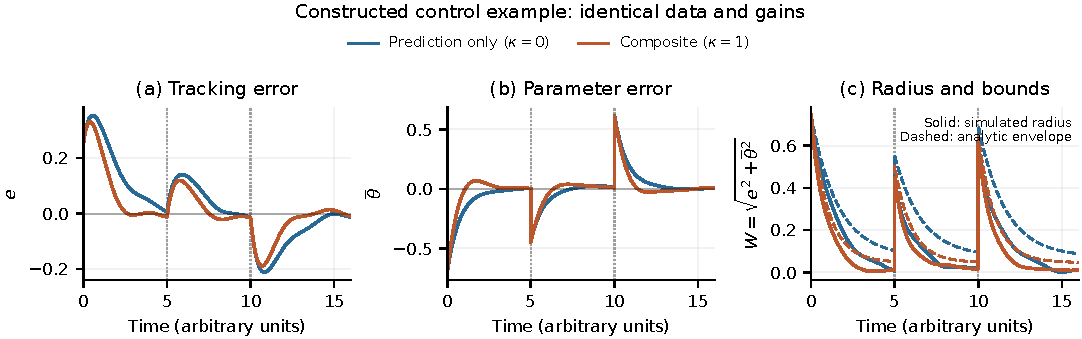
\includegraphics[width=\linewidth]{fig_theory_ood.pdf}
\caption{Constructed scalar control example. Prediction-only and composite
updates use identical gains and ideal current regression data. Dashed curves
are the analytic joint-error envelopes, with parameter-jump terms at times
5 and 10. This example isolates the tracking-feedback mechanism and is
separate from the reported VLA experiments.}
\label{fig:constructed}
\end{figure}

The constructed example has physical realization
$\dot q=u+\theta^*+d$, supplied target $r=0$, low-level feedback $k_0=-q$,
and feasible unrestricted command $u=-q-\hat\theta$. The same-command
nominal response satisfies $\dot\xi^{\rm nom}=-\xi^{\rm nom}$ with $\xi^{\rm nom}(0)=0$, hence
$\xi^{\rm nom}=0$. Thus $e=q$, $V_\xi=e^2/2$, and $\sigma_{\rm exec}=e$.
Its scalar error dynamics and update are
\begin{equation}
\begin{aligned}
\dot e&=-e-(\hat\theta-\theta^*)+.02\sin(2.3t),\\
\dot{\hat\theta}&=\kappa e+2(b_I-.65\hat\theta),
\qquad b_I=.65\theta^*+.006\sin(1.7t+.4).
\end{aligned}
\label{eq:constructed-system}
\end{equation}
with $e(0)=.25$, $\hat\theta(0)=0$, and
\begin{equation}
\theta^*(t)=\begin{cases}.7,&0\le t<5,\\
1.15-.03(t-5),&5\le t<10,\\.4,&10\le t\le16.\end{cases}
\end{equation}
The statistic $b_I$ is generated as an ideal current regression measurement,
with $H_I=.65$ throughout. The adaptive update receives that statistic, not
the unknown parameter directly. Both branches use identical information,
disturbances, and gains. This assumption isolates the adaptive feedback
mechanism; it makes no assertion about availability of comparable information
on a VLA task. Projection is inactive in this example.

The jump sizes are $+.45$ at $t=5$ and $-.6$ at $t=10$.
Between jumps, $|\dot\theta^*|\le.03$, so
$Q=\sqrt{.02^2+(2\cdot.006+.03)^2}=.0465188$.
The constant contraction metric is $M_c=1$. The weighted-certificate matrices are $K_{0,1}=\left[\begin{smallmatrix}1&-.5\\-.5&1.3\end{smallmatrix}\right]$
and $K_{1,1}=\operatorname{diag}(1,1.3)$.
We propagate the weighted envelope in Proposition~\ref{prop:gen-weighted} with $\tau=1$ on each interval and add the
jump norm at its boundary. The common drift bound also covers the
constant-parameter intervals and is conservative there.
\begin{center}\small
\begin{tabular}{lrr}
\toprule
Quantity & Prediction only & Composite\\
\midrule
Sufficient rate $\beta_{\kappa,1}$ & .627985 & 1.000000\\
Radius floor $Q/\beta_{\kappa,1}$ & .074076 & .046519\\
$\int_0^{16}e(t)^2dt$ & .292041 & .171081\\
$\int_0^{16}\tilde\theta(t)^2dt$ & .402695 & .298536\\
Peak $|e|$ & .353284 & .329610\\
\bottomrule
\end{tabular}
\end{center}
The trajectories use DOP853 with relative tolerance $10^{-11}$,
absolute tolerance $10^{-13}$, and maximum integration step $.025$.
Both satisfy the analytic envelopes on the evaluated time grid. The
composite parameter transient overshoots; a better joint tracking certificate is
not a pointwise ordering of parameter errors. The script
\code{audit/verify\_adaptive\_ood.py} regenerates the figure, trajectory
arrays, constants, and numerical checks without external data.

A second exact example illustrates conservatism. For
$\dot e=-.2e-\tilde\theta$, $\dot{\tilde\theta}=-.1\tilde\theta$,
the prediction-only system has eigenvalues $-.2,-.1$, but the unweighted
certificate has minimum eigenvalue $-.35249$. Choosing $\tau=.01$ in
Proposition~\ref{prop:gen-weighted} yields minimum eigenvalue $.07929>0$.
Thus a failed unweighted test cannot establish instability or a need for
control-error feedback. A separate stale-data check uses $H_I=2$ with
old parameter $.4$ and current parameter $1.1$, giving $\epsilon_I=-1.4$;
prediction adaptation to this old target converges to $.4$ despite positive
information. It is a data-validity diagnostic, not an evaluated reset scheme.

The script additionally checks 5,000 constructed inequalities for storage,
projection, and parameter jumps with heterogeneous gains. It also checks
500 stale-memory identities.
Finite numerical checks support consistency but do not replace the proofs
or validate their assumptions on the VLA experiments.

\subsection{Relation to the evaluated discrete observers}
\label{app:gen-discrete}
For calibrated additive observations $z_k=f_k+w_k$, take
$\Phi_k=I$ and $\theta^*=f$. Identification of offsets need not require
persistent command motion, conditional on a separately valid healthy
bias reference and identifiable residual sensitivity $S$. The innovation
law is a sampled prediction-gradient update with $H_{I,k}=I$, but its
state-dependent gain must be treated in the actual sampled proof. Its
error-to-truth recursion does not establish global pairwise Euclidean
contraction. The legacy observation-attenuated law targets $s_kz_k$ and
has effective prediction bias $(s_k-1)f_k+s_kw_k$. Under a fixed
noiseless input, it can contract to an incorrect physical target.
A gain estimator instead needs informative command regressors.
None of the documented VLA updates computes the $\kappa\sigma_{\rm exec}$ term.

The actual-law proofs in Appendix~\ref{app:implemented-theory} and
Appendix~\ref{app:theory} retain gates, projection, history, mask, and
applied snapshot age. Their coupled comparison is the sampled counterpart
of Proposition~\ref{prop:prediction-comparison}; this connection does not
replace checking those implementation conditions.

For completeness, a continuous-time bound supports an Euler claim only
under additional structure. For a constant true parameter and a constant
quadratic composite metric let
$z=(P^{1/2}e,\Gamma^{-1/2}\tilde\theta)$, and suppose the implemented
joint map is exactly
\begin{equation}
 z_{k+1}=\Pi_{\mathcal Z}[z_k+h\mathcal F_k(z_k)+h\delta_k],\quad
 0\in\mathcal Z,\quad \|\delta_k\|\le\bar\delta,
 \label{eq:gen-euler}
\end{equation}
where $\mathcal Z=\R^{\dim e}\times
\Gamma^{-1/2}(\Theta-\theta^*)$ is closed and convex. If
$z^\top\mathcal F_k(z)\le-\beta\|z\|^2$ and
$\|\mathcal F_k(z)\|\le L\|z\|$ on the relevant domain, then
\begin{equation}
 \|z_k\|\le q_h^k\|z_0\|+
 \frac{h\bar\delta}{1-q_h}(1-q_h^k),\quad
 q_h=\sqrt{1-2\beta h+L^2h^2}<1,
 \quad 0<h<2\beta/L^2.
 \label{eq:gen-euler-bound}
\end{equation}
Projection is nonexpansive and fixes zero; expanding
$\|z+h\mathcal F_k(z)\|^2$ gives the factor and summing the scalar
recursion proves the claim. A physical sampled plant or chunked policy
usually has a different map and needs an explicit discretization defect
or a direct discrete storage inequality. Increasing gains can increase
$L$ as well as $\beta$, tightening the step-size restriction. This
illustration does not certify the experimental control rate.
